\documentclass{acm_proc_article-sp}

% Parts of the style depend on whether a PDF or a DVI output is created.
\usepackage{ifpdf}

\usepackage{amsfonts}
\usepackage{amsmath}
%\usepackage{amsthm} % Redefines `proof`.
\usepackage{courier}
\usepackage[english]{babel}

% Include graphics.
\usepackage{graphicx}
\ifpdf
  % Declare the supported file extensions.
  \DeclareGraphicsExtensions{.jpg,.mps,.pdf,.png}
\fi

\usepackage{helvet}
\usepackage[utf8]{inputenc}
\usepackage{times}
\usepackage{verbatim}
\usepackage{url}
\newcommand{\URL}[1]{{\small \url{#1}}}
\usepackage{enumitem}

% Operator macros.
\newcommand{\absolute}[1]{\lvert#1\rvert}
\newcommand{\bigsetdef}[2]{\big\{#1\,\,\big\vert\,\,#2\big\}}
\newcommand{\card}[1]{\lvert#1\rvert}
\newcommand{\equivpair}[2]{#1 \approx #2}
\newcommand{\equivset}[1]{[#1]_{\approx}}
\newcommand{\higherapprox}[0]{\overline{\approx}}
\newcommand{\interp}[1]{#1^{\mathcal{I}}}
\newcommand{\lowerapprox}[0]{\underline{\approx}}
\newcommand{\natnum}[1]{#1 \in \mathbb{N}}
\newcommand{\pair}[2]{\langle#1,#2\rangle}
\newcommand{\powerset}[1]{\mathcal{P}(#1)}
\newcommand{\range}[2]{#1,\ldots,#2}
\newcommand{\set}[1]{\{#1\}}
\newcommand{\setdef}[2]{\{#1\,\vert\,#2\}}
\newcommand{\setrange}[2]{\{#1,\ldots,#2\}}
\newcommand{\triple}[3]{\langle#1,#2,#3\rangle}
\newcommand{\tuple}[1]{\langle#1\rangle}
\newcommand{\tuplerange}[2]{\langle#1,\ldots,#2\rangle}

% Operator declarations
\DeclareMathOperator{\indpo}{{\mathbb{IND}-\mathbb{PO}}}
\DeclareMathOperator{\indp}{{\mathbb{IND}-\mathbb{P}}}

% Theorem styles.
\newtheorem{assumption}{Assumption}
\newtheorem{axiom}{Axiom}
\newtheorem{convention}{Convention}
\newtheorem{example}{Example}
\newtheorem{definition}{Definition}
\newtheorem{lemma}{Lemma}
\newtheorem{principle}{Principle}
\newtheorem{proposition}{Proposition}
\newtheorem{specification}{Specification}
\newtheorem{statement}{Statement}
\newtheorem{theorem}{Theorem}

%terms
\newcommand{\obs}{LOB Observer}

\begin{document}

\title{
  A Web Observatory for the Machine Processability of
   Structured Data on the Web
}

\numberofauthors{4}

\author{
\alignauthor
  Wouter Beek\\
  \affaddr{VU University Amsterdam}\\
  \affaddr{De Boelelaan 1081a}\\
  \affaddr{Amsterdam, The Netherlands}\\
  \email{w.g.j.beek@vu.nl}
\alignauthor
  Paul Groth\\
  \affaddr{VU University Amsterdam}\\
  \affaddr{De Boelelaan 1081a}\\
  \affaddr{Amsterdam, The Netherlands}\\
  \email{p.t.groth@vu.nl}
\alignauthor
  Stefan Schlobach\\
  \affaddr{VU University Amsterdam}\\
  \affaddr{De Boelelaan 1081a}\\
  \affaddr{Amsterdam, The Netherlands}\\
  \email{k.s.schlobach@vu.nl}
\and
\alignauthor
  Rinke Hoekstra\\
  \affaddr{VU University Amsterdam}\\
  \affaddr{De Boelelaan 1081a}\\
  \affaddr{Amsterdam, The Netherlands}\\
  \email{rinke.hoekstra@vu.nl}
}

\maketitle
\begin{abstract}
General human intelligence is needed in order to process content
 on the Web of Documents.
On the Web of Data (WOD), content is intended to be
 machine-processable as well.
But the extent to which a machine is able to navigate, access,
 and process the WOD has not been extensively researched.
%How friendly is today's Web of Data for machines?
We present \obs, a web observatory that studies the Web
 from a machine processor's point of view.
We do this by reformulating the five star model
 of Linked Open Data publishing
 in quantifiable terms.
Secondly, we built an infrastructure that allows
 the model's criteria to be quantified over existing datasets.
Thirdly, we analyze a significant snapshot of the WOD
 using this infrastructure and discuss the main problems
 a machine processor encounters.
\end{abstract}

% A category with the (minimum) three required fields
\category{E.}{Data}{Miscellaneous}
%A category including the fourth, optional field follows...
\category{H.3.5}{Online Information Services}{Web-based services}

\terms{Measurement, Standardization}

\keywords{Web Observatory, Machine processing, Web of Data, Linked Open Data}

\section{Introduction}
\label{sec:introduction}

Identity relations are a cornerstone of logic-based knowledge representation.
They allow to state and relate properties of an object
  using multiple names for that object, and conversely,
  they allow to infer that different names actually refer to the same object.

In particular, identity relations are
  at the foundation of the Linked Open Data initiative
  and the Semantic Web (SW) in general \cite{BizerCyganiakHeath2007}.
The SW consists of many different sets of assertions
  that are published on the Web by different authors in different locations,
  often using different names for the same object.
Identity relations then allow the interlinking of these multiple descriptions
  of the same thing.
For example, statements about Amsterdam in the DBpedia dataset
  (where Amsterdam is referred to as
  \URL{http://dbpedia.org/resource/amsterdam}, abbreviated as
  \URL{dbp:amsterdam})
  can be combined with statements about Amsterdam in GeoNames
  (where Amsterdam is referred to as
  \URL{http://sws.geonames.rg/2759794}), by asserting identity between
  these two names.

However, the traditional notion of identity
  (expressed by \texttt{owl:sameAs} \cite{MotikPaterschneiderGrau2012})
  is often problematic, e.g. when objects are considered the same in some
  contexts but not in others.
The standing practice in such cases is to use weaker relations of relatedness
  (e.g., \texttt{skos:related} \cite{MilesBechhofer2009}).
Unfortunately, these relations suffer from the opposite problem of having
  almost no formal semantics, thereby limiting reasoners
  in drawing inferences.

According to the traditional semantics of the identity relation,
  identical terms can be replaced for one another in all non-modal contexts
  \emph{salva veritate}.
Practical uses of \texttt{owl:sameAs} are known to violate this
  strict condition
  \cite{HalpinHayes2010,HalpinHayesMccuskerMcguinnessThompson2010}.

\begin{comment}
The SW is not only a formal model,
  but is also a social component that evolves over time,
  i.e. it is a social machine cite{Www2013}.
Being a social and symbolic system at the same time,
  meaning on the SW is denoted by its semantics as well as its pragmatics.
\end{comment}

\subsection{Outline}

In the following section,
  we will analyze in some more detail the problems that
  are caused by the traditional notion of identity, both in general,
  and in the SW setting in particular.
After surveying existing work on these problems
  in section \ref{sec:related_work},
  we will then present our approach to the problem of identity
  in section \ref{sec:approach}.
First at a very high level and then in more formal detail.
We illustrate the results of applying our formalism to
  a realistic heterogeneous SW dataset.
In sections \ref{sec:implementation} and \ref{sec:experimental_design}
  we put our formalism to the test
  in an experimental setting,
  showing that it behaves as required.

\section{Related work}
\label{sec:related_work}

Existing research suggests six different solutions for
  the problem of identity on the SW.

\textbf{[1] Introduce weaker versions of {\small \texttt{owl:sameAs}}}
  \cite{HalpinHayes2010,MccuskerMcguinness2010}.
Candidates for replacement are
  the SKOS concepts
  {\small \texttt{skos:related}} and {\small \texttt{skos:exactMatch}}
  \cite{MilesBechhofer2009}.
The former is not transitive,
  thereby limiting the possibilities for reasoning.
The latter is transitive,
  but can only be used in certain contexts.
It is not defined in what contexts it can be used
  \cite{MilesBechhofer2009}.\footnote{
    For instance, the property {\small \texttt{skos:exactMatch}}
    ``is used to link two concepts, indicating a high degree of confidence
    that the concepts can be used interchangeably across a wide range of
    information retrieval applications.''
  }
\begin{comment}
% SIMILARITY
The problem with using weaker notions such as relatedness,
  is that everything is related to everything in \emph{some} way.}
% Shall we discuss similarity here as well?
% Does similarity differ from relatedness?
\end{comment}

\textbf{[2] Restrict the applicability of identity relations}
  to specific contexts.
In terms of Semantic Web technology, identities are expected to hold
  within a named graph or within a namespace,
  but not necessarily outside of it \cite{HalpinHayes2010}.
\cite{Melo2013} has successfully used the Unique Names Assumption
  within namespaces in order to identify many (arguably) spurious
  identity statements.

\textbf{[3] Introduce additional vocabulary} that does not weaken but extends
  the existing identity relation.
\cite{HalpinHayes2010} mention an explicit distinction that could be made
  between mentioning a term and using a term,
  thereby distinguishing an object and a Web document describing that object.
Other possible extensions of {\small \texttt{owl:sameAs}} might take
  the Fuzzyness and/or uncertainty of identity statements into account.

\textbf{[4] Use domain-specific identity relations}
  \cite{MccuskerMcguinness2010}.
For instance
    ``$x$ and $y$ have the same medical use''
  replaces
    identity in the domain of medicine,
and
    ``$x$ and $y$ are the same molecule''
  replaces
    identity in the domain of chemistry.
The downside to this solution is that domain-specific links are
  only locally valid, thereby limiting knowledge reuse.

\textbf{[5] Change the modeling practice}, possibly in a (semi-)automated way
  by adapting visualization and modeling toolkits to produce notifications
  upon reading SW data, or by posing additional restrictions on the creation
  and alteration of data. For example, adding an RDF link could require
  reciprocal confirmation from the maintainers of the respective datasets.
  \cite{HalpinHayes2010,DingShinavierFininMcguinness2010}
The problem with introducing checks on editing operations,
  is that it violates one of the fundamental underpinnings of the SW;
  namely that on the Web of Data anybody is allowed to say
  anything about anything \cite{AntoniouGrothHarmelenHoekstra2012}.

\textbf{[6] Extract network properties of {\small \texttt{owl:sameAs}}
  datasets} \cite{DingShinavierShangguanMcguinness2010}.
Although this work shows that network analysis can provide insights
  into the ways in which identity is used in the SW,
  these endeavors have not yet been related to the semantics of the
  identity relation.
We believe that utilizing network theoretic aspects in order to
  determine the meaning of identity statements
  would be interesting future research.

What the existing approaches have in common is
  that quite some work has to be done
  (adapting or creating standards, instructing modelers, converting existing
  datasets) in order to resolve only some of the problems of identity.
Our approach provides a way of dealing with the heterogeneous real-world
  usage of identity in the SW that is fully automated and requires
  no changes to standards, modeling practices, or existing datasets.


\section{Operationalization of the five star model}
\label{sec:operationalization}

This section gives an operationalized interpretation of
 the five star model of LOD publishing.
The original formulation of the model \cite{Bernerslee2006}
 is displayed in Table \ref{tab:five_star}.
Our goal is to make the model concrete enough in order to be able to
 quantify adherence to it.

\begin{table}
  \label{tab:five_star}
  \caption{Five Star Linked Open Data}
  \centering
  \begin{tabular}{|l|l|}
    \hline
        $\star$
      & Available on the web (whatever format) but with \\
      & an open license, to be Open Data.\\
    \hline
        $\star\star$
      & Available as machine-readable structured data \\
      & (e.g. excel instead of image scan of a table).\\
    \hline
        $\star\star\star$
      & as (2) plus non-proprietary format \\
      & (e.g. CSV instead of excel).\\
    \hline
        $\star\star\star\star$
      & All the above plus, Use open standards from W3C to \\
      & identify things, so that people can point at your stuff.\\
    \hline
        $\star\star\star\star\star$
      & All the above, plus: Link your data to other people's \\
      & data to provide context.\\
    \hline
  \end{tabular}
\end{table}

\begin{principle}[First star]
\label{principle:first_star}
  Available on the web (whatever format) but with an open license,
   to be Open Data.
\end{principle}

\subsubsection*{`stuff'}

The use of the mass noun `stuff` in principle \ref{principle:first_star}
 suggests that what is made available on the Web cannot be readily counted.
Since we want to quantify over data on the Web,
 we replace this word with a count noun
 that allows discrete units to be denoted.
Two replacements seem viable here: datasets and individual parts
 (e.g. files, endpoints) or `resources' that constitute datasets.
We choose resources here,
 because several linked data properties are not defined on datasets,
 but on individual parts.
We define resources as digital entities that have
 been purposefully published with the intent of being (potentially)
 disseminated as some form of partially or completely
 machine-processable data.

\subsubsection*{`Web'}

The Web is interpreted to denote the collection of documents
 (some of them containing data) that are accessable on the Internet.
We restrict ourselves to those parts of the Internet that are
 readily accessable -- i.e. without authentication --
 over TCP/IP by using a standardized Internet protocol
 (mainly FTP and HTTP(S)).

\subsubsection*{`make available'}

There are various aspects to making resources available on the Web.
Availability of a resource for a machine agent means that
 the agent is able to
 (1) locate the resource,
 (2) connect to the host that disseminates the resource, and
 (3) retrieve the resource from the host.

A resource is universally locatable if there exists a resource locator
 that denotes the resource's location
 and this locator can be readily found by a machine agent.
Resource locators have to be supplied to the agent.
This cannot always be done in an automated fashion.
We therefore use a hand-made, curated catalogue of resource locators
 for the automated to use (see section \ref{sec:implementation}).

Findability of the location presupposes the location exists
 and that there is some apparatus residing at that location that is able
 to serve the resource located there.
On the Web existence is a transient notion,
 as locations go in and out of existence all of the time.

The ability of the apparatus at the findable location to serve
the resource consists of
 (3.1) it being responsive to requests from outside,
 (3.2) its ability to interpret requests based on
 the standardized communication protocol that is indicated in
 the universal locator (the so-called `scheme' part of the locator), and
 (3.3) its ability to respond to a correctly formulated request
 in a reply that is itself correctly formulated according to the same
 communication protocol.

As before, we exclude those cases in which it is necessary
 to authenticate and/or use a non-automated way
 of retrieving the resource.
This explicitly excludes content for which a form has to be filled in
 or an account has to be creating by a human user
 in order to gain access.

\subsubsection*{`open license'}

We interpret the requirement of being made available under an open license
 as being made available under a license that is defined by
 the Open Data Commons\footnote{\url{http://opendatacommons.org/}} \cite{miller2008open},
 and that is compliant with either
 the Open Knowledge Foundation's Open Definition\footnote{\url{http://opendefinition.org/od/}}
 or the Open Source Initiative's
 Open Source Definition\footnote{\url{http://opensource.org/license}} \cite{rosen2004open},
 or both.

\begin{principle}[Second star]
  \label{principle:second_star}
  Available as machine-readable structured data
   (e.g. excel instead of image scan of a table).
\end{principle}

\subsubsection*{`structured data'}

For principle \ref{principle:second_star} we interpret
 the structuredness of data as a gradient property,
 and define the amount of structure a collection of data possesses
 as the set of relational operators that are supported by
 the ``common'' implementations of query languages
 over that data.\footnote{The appeal to common implementations
  is needed to rule out exotic cases such as the application
  of set operators on image data.}

This interpretation is difficult to operationalize due to the variety of
 relational operators and the absence of a formal definition of
 ``being common'' or ``being a common implementation''.
Still this interpretation allows us to distinguish between
 an Excel table and an image of the same table,
 since the former allows more queries to be performed than the latter
 (e.g. ordering of rows by the values in the first column,
  summation of the values in the respective columns).

\begin{principle}[Third star]
  \label{principle:third_star}
  as (2) plus non-proprietary format (e.g. CSV instead of excel).
\end{principle}

\subsubsection*{`non-proprietary'}

For principle \ref{principle:third_star} we have not found
 an authoritative source that
 enumerates the open and proprietary formats respectively,
 not even for the common IANA-registered MIME types.
We therefore interpret the proprietary nature of structured data formats
 based on common knowledge that is findable on the Web.

\begin{principle}[Fourth star]
  \label{principle:fourth_star}
  All the above plus, Use open standards from W3C (RDF and SPARQL)
   to identify things, so that people can point at your stuff.
\end{principle}

The use of open standards could  potentially be quantified by the number of
 syntax errors that occur when loading
 a data file in a standards-conformant tool.
However, in practice it is not easy to find tools that are fully
 standards-compliant, and tools differ on the number of erorrs
 they check for an emit.
To lower the dependence on specific tools,
 we do not count the number of syntax errors reported
 but the number of imported triples instead.

We initially wanted to quantify principle \ref{principle:fourth_star}
 by stating that all triples in a dataset ought to be parsable
 and loadable in a triple store.
But we could not find a reliable method for assessing
 the number of triples that is (or should be) present
 in a resource.\footnote{E.g. our investigation showed that
   netiher the CKAN \texttt{size} property
   the number of triples reported in VoID description
   can be used for this, see section \ref{sec:implementation}.}
We therefore decided to interpret successfully passing
 Principle \ref{principle:fourth_star} as
 being able to load some triples (i.e. one or more).


\section{Implementation}
\label{sec:implementation}

Using our operationalization of the five star model of data sharing
 in section \ref{sec:operationalization} we created
 a web observatory for linked open data,
 called \obs.\footnote{Code and results available at
   \url{https://github.com/wouterbeek/LODObs}}

\obs uses an automated script in order to look for
 data on the Web.
The script must be given a set of locations where Web data
 is likely to be found.
For this we use CKAN API.\footnote{\url{http://docs.ckan.org}}
CKAN is an open-source data portal platform
 that allows datasets that are published on the Web to be catalogued.
There are various catalogues available,
 including the governmental initiatives towards data sharing
 of the UK and the USA.

\obs gives a tabular overview of the results of
 processing the various resources, see Figure \ref{fig:lod_observer}.
\obs provides more detailed information than we are able to give
 in our results section (i.e. section \ref{sec:results});
 e.g. it shows the specific error messages encountered
 and the syntax error that occur while reading a serialization format.

\begin{figure*}[th!]
  \label{fig:lod_observer}
  \centering
  \includegraphics[width=0.85\textwidth]{./img/table}
  \caption{
    A part of the table that is generated by \obs.
    Each row in the table displays the results of retrieving a single
     resource from Datahub.
    Each column in the table corresponds to a specific action
     that is performed for a specific resource.
    The picture shows the results of executing the following four actions
     for three resources:
     (1) downloading the resource,
     (2) unarchiving it,
     (3) determining the file size, and
     (4) counting some basic VoID statistics \cite{Void2011}.
  }
\end{figure*}

\subsubsection*{Locating resources}

CKAN uses URLs as universal locators for resources.
URLs are URIs that identify a resource via a representation of
 its primary access mechanism or scheme (e.g. HTTP)
 and its network location (e.g. \texttt{www.datahub.io})
 that can be accessed using standardized operations
 defined for that scheme. \cite{Rfc3305}

The datasets that are catalogued by CKAN provide
 a starting point for an automated agent to search for data on the Web,
 since all data registrations can be queried using an API.
Since datasets have to be explicitly registered at a CKAN catalogue,
 this ensures that they are purposefully published
 as machine-processable data,
 thereby following our definition of a `resource'
 (see section \ref{sec:operationalization})
Each CKAN resource has a URL property field,
 which allows an automated agent to find a URL string for each resource.

\subsubsection*{Connecting to disseminating host}

When using the URL string to locate a resource we find that
 not all URL strings parse according to the grammar
 in the URL specification \cite{Rfc3986},
 and some URLs that are grammatically correct contain a scheme
 that is not registered with
 the Internet Assigned Numbers Authority
 (IANA).\footnote{\url{http://www.iana.org/assignments/uri-schemes/uri-schemes.xhtml}}
%\footnote{
%  The number of resources for which the URL string parses correctly
%  can be increased by trimming leading and trailing whitespace (US-ASCII 32)
%  and by prepending the string with a commonly occurring scheme descriptor
%  (e.g., \texttt{http://}) in case the grammar cannot detect a scheme.
%}

Culprits:
\begin{itemize}[noitemsep,nolistsep]
  \item The URL string does not parse according to the RFC grammar.
  \item The parsed URL string does not contain an IANA-registered scheme.
\end{itemize}

For URLs that are grammatically correct an automated agent is able to
 verify whether there exists a host authority at the location
 denoted by the URL.
As with the Web of Documents, this is not always the case,
 resulting in a ``host not found exception''.
Once a host authority is found, it has to accept a connection
 with the automated agent.
Only when a connection is established can the agent send its request
 to the authority.
The agent and authority both have to maintain the connection
 for the duration of the subsequent request/response-interaction.

Culprits:
\begin{itemize}[noitemsep,nolistsep]
\item The host that is denoted by the URL's authority string cannot be found.
\item The connection was refused by the host.
\item The connection was neither refused nor accepted by the host.
\item The connection was established, but was broken off
      during subsequent communication.
\item The host was redirecting the connecting agent indefinitely.
\end{itemize}

\subsubsection*{Retrieving resource from host}

Once a reliable connection between agent and host is established
 for the duration of a communicative interaction,
 the agent is able to send a request in one of
 the standardized Internet communication protocols.
Specifically, \obs supports communications via FTP and HTTP(S).

Various things can go wrong in both formulating the request and
 in replying to it.
This results in various status codes that denote different problems
 that cause the communication to be ineffective.

\subsubsection*{Open license}

Many CKAN registered resources have a license property.
The licenses are similar to those defined by the Open Data Commons,
 but some mismatches occur.
In the Datahub CKAN repository, 33 licenses are used,
 18 of which are underdefined (i.e., with no semantic description),
 impacting 5\% of the resources.
We have added manual mappings from the CKAN licenses onto
 the repository of Open Data Commons license descriptions.
%This results in added descriptions for 14 underdefined licenses,
% additional properties for 4 licenses that were already partially defined,
% and leaves only 2 underdefined licenses that have been equated to
% `license' \texttt{ckan:None} using \texttt{owl:sameAs} statements.

Culprits:
\begin{itemize}[noitemsep,nolistsep]
\item Has no license string.
\item Has a license string that cannot be mapped to
       a license that occurs in
       the Open Data Commons license description set.
\item Has a recognized license that is not open.
\end{itemize}

\subsubsection*{Structured \& non-propetary}
\label{sec:implementation_mime}

In order to implement the structuredness requirement,
 we have manually classified the MIME types that occur in the CKAN catalogue
 into `structured' and `unstructured' ones.
This goes against our interpretation of structuredness as
 a gradient property, but the partial order constituted by the relation
 ``supports at least the same set of relational operators''
 cannot be easily established in an automated way,
 as this would require a model of query operators
 and a description of MIME types in terms of the operators that are
 supported by those content types.

We list the 4 ways in which we can check for a resource's content type
 in CKAN, annotated with the number of resources for which
 this type can be retrieved:
\begin{itemize}[noitemsep,nolistsep]
  \item The value of the CKAN \texttt{mimetype} property.
        Present for 6,332 resources (45\%).
  \item The value of the CKAN \texttt{format} property
        Present for 10,226 resources (73\%).
  \item The MIME type in the HTTP \texttt{Content-Type} response header
         (not present in CKAN).
  \item The extension of the resource file.
\end{itemize}

We are specifically interested in linked data,
 but not all linked data serialization formats have a MIME type
 that is registered by IANA.
Moreover, some of the registered linked data content types are deprecated.
We take both deprecated and current MIME types into account,
 and officially registered ones as well as ones that are
 de facto being used to denoted linked data.
Not all MIME types that occur in CKAN repositories are valid,
 some of them seem to be typos/variants of existing MIME types
 for which we have added mappings manually.

The values of the CKAN \texttt{format} property are not standardized
 and are also manually mapped onto IANA-registered and de facto used
 MIME types.
Some of the format values seem to be typographic variants
 of each other (impacting 96 resources).
For some format values no mapping to an existing MIME type
 could be found (impacting 52 resources).

%The MIME type that occurs in the \texttt{Content-Type} response header
% is not always the same as the MIME type denoted by either the
% \texttt{format} or the \texttt{mimetype} property.
%Sometimes this is more generic or a more specific than
% the CKAN-registered value (XX\%),
% but sometimes it is another value altogether.

File extensions were not mapped to content type,
 because of the absence of a straightforward mapping.
We do not believe file extensions are a reliable indicator
 of a resource's format.

A special case occurs for resources that are compressed
 in some archive format.
For these neither MIME type, format, nor Content-Type header
 are indicative of the uncompressed content,
 so for these we have to rely on the file extension.

When none of the above enumerated methods works,
 we can try to parse a file's first few lines.
This is generally quite difficult because of the large number
 of different formats, encoding types, and syntactic error that may occur.
In the general case we are only able to make a best guess at
 a resource's format.

Culprits:
\begin{itemize}[noitemsep,nolistsep]
  \item The resource's type is not set.
  \item The resource's type is set, but it does not map to a MIME type
         that is registered by IANA and it is not one of the MIME types
         in the list of de facto used identifiers of LOD content.
  \item The resource's type can be mapped to an IANA-registered type
         or a de facto LOD type, but it does not denote structured data.
  \item The resource's type can be mapped to an IANA-registered type
         or a de facto LOD type, but it denotes a proprietary format.
\end{itemize}

\subsubsection*{Syntactic correctness: readable triples}

We use SWI-Prolog's Semweb library \cite{wielemaker2003}
 for loading the resources into a triple store.

The number of triples that can be loaded is often inconsistent with
 the value of the CKAN \texttt{size} property.\footnote{The CKAN
    \texttt{size} property is often taken to represent the actual number
    of triples in a dataset.
   For example, the famous visualizations of the LOD cloud make use of
    the values for this property.
   Our observatory shows that these visualizations are not always based
    on the correct numbers.}

Culprits:
\begin{itemize}[noitemsep,nolistsep]
  \item From the resource no triples can be read.
  \item From the resource some triples are read (syntax errors).
  \item From the resource all triples are read (no syntax error).
\end{itemize}


\section{Results}
\label{sec:results}

In this section we enumerate the statistics for our sample of
 Linked Open datasets that we validated according to
 the operationalized five star criteria described in
 section \ref{sec:operationalization}.

We have run the implementation described in section \ref{sec:implementation}
 on a specific CKAN repository: Datahub.
Datahub is a portal for registering open datasets,
 mostly coming from the academic domain.
For instance, it includes the ``LOD cloud'' group,
 which is a collection of linked and open datasets
 that are sometimes taken to `stand for' or `represent'
 the WOD.\footnote{This claim is not correct;
  the WOD and the LOD cloud are much bigger, as our approach shows.}

In order to run our implementation more efficiently,
 we have swapped the second and third star with the first one,
 since our implementation is able to assess whether a dataset
 is structured and non-proprietary without having to download it
 (using CKAN properties).

Since CKAN entries can be updated by their maintainers and
 hosts that were offline during the execution of our \obs script
 may go online at some later point in time,
 the results we give here are a snapshot of a significant subset
 of the WOD at a specific moment in time.

Our implementation was run without human intervention,
 except for the hand-made lists of MIME types
 for structuredness and proprietariness
 (see section \ref{sec:implementation_mime}),
 thereby allowing us to assess the number of resources
 that is findable, retrievable, and processable by a machine agent.

%\subsubsection*{Taking a LOD sample}

Datahub contains 13,940 descriptions of resources,
 11,579 (83,1\%) of which have either a MIME type or
 a format that can be mapped onto a MIME type
 (see section \ref{sec:implementation}).
Based on these MIME types, we take as our sample all the resources
 that can be associated with a MIME type that denotes linked data.
This sample consists of 2,369 resources or 17,0\% of all the resources
 in Datahub.

%\subsubsection*{Statistics for LOD resources}

%One universal locator contains a scheme that is not registered with IANA.
In the rest of this section, all percentages are relative to
 the LOD sample of 2,369 resources mentioned above,
 unless explicitly stated to be determined otherwise.
From this sample 2,123 resources (89,6\%) \obs is able to connect to
 the resource's host.
Table \ref{tab:findability} enumerates the number and percentage
 of resources that encounter the various culprits
 with respect to connecting to a resource's host.

\begin{table}
  \centering
  \caption{Resources whose host cannot be connected to.}
  \label{tab:findability}
  \begin{tabular}{|l|l|l|}
    \hline
    \textbf{Culprit} & \textbf{Numb.} & \textbf{Perc.} \\
    \hline
    \hline
    Cannot connect to host & 76 & 3,2\% \\
    \hline
    Host was found, but connection was rejected & 14 & 0,6\% \\
    \hline
    Establishing connection timed out  & 12 & 0,5\% \\
    \hline
    Caught in redirection loop & 115 & 4,8\% \\
    \hline
    Connection timed out while reading data & 48 & 2,0\% \\
    \hline
    %Try again? & 8 & 0,3\% \\
    %\hline
  \end{tabular}
\end{table}

For 2,001 LOD resources (84,5\%) \obs is able to retrieve
 the data file.
Table \ref{tab:retrievability} enumerates the number and percentage
 of resources that encounter the various culprits
 with respect to retrieving resources from their host.

\begin{table}
  \centering
  \caption{Resources that cannot be retrieved from host.}
  \label{tab:retrievability}
  \begin{tabular}{|l|l|l|}
    \hline
    \textbf{Culprit} & \textbf{Numb.} & \textbf{Perc.} \\
    \hline
    \hline
    Bad Request (400) & 9 & 0,4\% \\
    \hline
    Unauthorized (401) & 4 & 0,2\% \\
    \hline
    Forbidden (403) & 14 & 0,6\% \\
    \hline
    Not Found (404) & 295 & 12,5\% \\
    \hline
    Not Acceptable (406) & 14 & 0,6\% \\
    \hline
    Conflict (409) & 1 & 0,004\% \\
    \hline
    Internal Server Error (500) & 38 & 1,6\% \\
    \hline
    Bad Gateway (502) & 1 & 0.0004\% \\
    \hline
    Service Unavailable (503) & 19 & 0,8\% \\
    \hline
  \end{tabular}
\end{table}

For 1,719 LOD resources (72,6\%) the HTTP response contains
 a \texttt{Content-Type} header with a legal MIME content type.
For 603 (25,5\%) LOD resources for which the response contains
 a \newline\texttt{Content-Type} header,
 the MIME type is different from the one that occurs
 in CKAN's meta-description of the resource.

247 (10,4\%) LOD resources are archived files,
 46 (18,6\% ofthe archived resources) of which cannot be unpacked
 by standard archive tools.
%This brings the number of files for which the MIME type is consistent
% and that can be unpacked in case it is an archive,
% to 1,070 (45,2\%).

Parallel to the problem of retrieving LOD resources,
 there is the problem of validating the licensing conditions.
For the sample of 2,369 resources \obs retrieved,
 540 (22.8\%) did not have a license associated with it.
 240 (10.1\%) resources have a closed license,
 and 1,615 (68.2\%) resources have an open license.

When we combine the retrievability of the data with the licensing conditions,
 we have 1,203 (50,8\%) resources,
 that result in over 668 Gigabytes of
 downloaded (purported) linked open data files.

% Of the intersection we can load about 74\%.
Not all these files are syntactically well-formed.
The script can load some triples (i.e. one or more) for 891 resources,
 or 37,6\% of the original sample.
The success criteria for each of the above described steps is displayed
 in Figure \ref{fig:stairs}.

\begin{figure*}[th!]
  \label{fig:stairs}
  \centering
  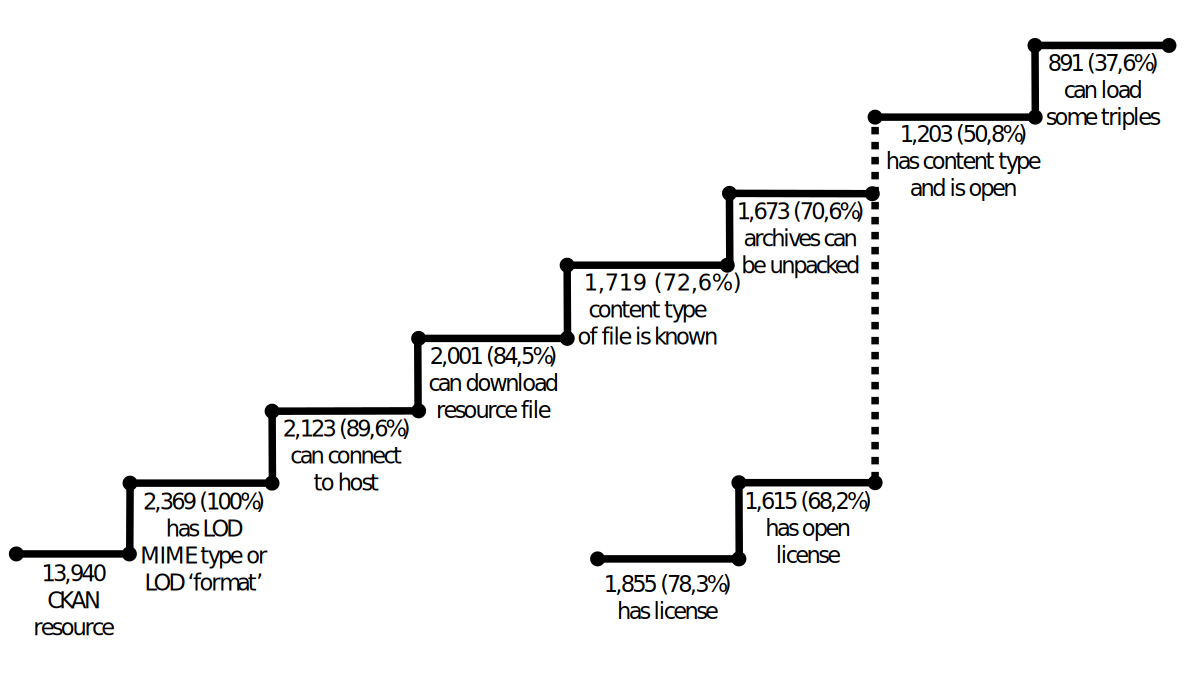
\includegraphics[width=0.9\textwidth]{./img/stairs}
  \caption{
    A `staircase' overview of the succes rates of the various tasks
     a machine agent has to perform in order to retrieve
     linked open data.
    The second stair from the left is the sample we have chosen to
     run our script on (set to 100\%);
     the percentages that appear in the other stairs are relative
     to this number.
    The stair in the top right corner shows that 37,6\% of
     the Datahub resources are fully machine-processable.
  }
\end{figure*}

%Maybe one or two diagram that show that success rates are conditional on
% e.g. domain (scientific versus governmental),
% sientific domain (medical versus rest),
% or ...



\section{Discussion}
\label{sec:discussion}

Here, we discuss possible reasons for the results presented
 in section \ref{sec:results}.
As the Web is a socio-technical construct,
 we focus not only on technical reasons for lack of machine processability
 but also on social reasons.

Technically, we see many of the common errors identified by
 the Pedantic Web group\footnote{See~\cite{conf/www/HoganHPDP10} and
   Frequently Observed Problems on the Web of Data: \url{http://pedantic-web.org/fops.html}}.
Many of these come from difficulties in configuring Web Servers
 or appropriately applying standards for access.
For example, setting up content-negotiation is often difficult;
 even making sure content-types are properly defined.
We also believe that many simple syntax errors stem from
 the use of common UNIX text manipulation tools
 (e.g. \texttt{grep}, \texttt{sed}).
This is evidenced by our own experience talking to developers
 as well as investigating some of the datasets by hand.
Also, the mismatch between actual content and file extension
 widely occurs because of multiple flavors of RDF, in particular,
 many of the text formats overlap (e.g. is it a Trig or Turtle serialization?).

It is important to note that issues with providing quality data
 are not necessarily a function of Linked Data formats (i.e. RDF).
Most data scientists can easily attest to the difficulties
 in processing data \cite{baddatabook}.
These vary from data being designed for human consumption\footnote{e.g.
  Laid out in a spreadsheet to be visually appealing
  and not to be processed.}
 to being encoded in a difficult to parse format.\footnote{e.g.
  A CSV file provided as a PDF.}
The site \url{http://okfnlabs.org/bad-data/} provides several examples
 of machine unfriendly data.

Much of these technical issues have to do with lack of tooling
 for both data consumption as well as publication.
For instance the Billion Triple Challenge\footnote{\url{http://km.aifb.kit.edu/projects/btc-2012/}}
 contains many files that cannot be loaded by any standards-compliant tool.
Many of these bigger data dumps seem to have only been processed
 by text tools, i.e. without fully parsing the syntax of
 the data serialization language.
At the same time, we are still far from the current state that we have
 on the Web of Documents, where we have sophisticated programs
 that are tolerant of errors in data (e.g. Web Crawlers and Browsers).
Nor do we have a similar rich environment of guidelines
 and tools for publication
 (e.g. Webmaster guidelines\footnote{\url{https://support.google.com/webmasters/answer/35769?hl=en}},
  content publishing platforms\footnote{\url{http://wordpress.org}}).

Importantly, these technical issues cannot be separated from
 the social environment that data publication resides in.
Data publication -- and in particular Linked Data publication --
 has numerous social issues that impact both its quality
 and availability for use by machines.
For example, those datasets with established communities
 have a better chance for staying up:
 biological and chemical datasets in their Linked Data form
 are generally of better quality.
They are often backed by organizations who have as a purpose
 making such resources available, for example,
 the European Bioinformatics Institute,
 the National Center for Bio-ontology,
 or the Swiss Institute for Bioinformatics.
They also have the requisite expertise and financing for
 maintaining this data\footnote{See for example,
   the EBI RDF platform \url{http://www.ebi.ac.uk/rdf/about-rdf-platform}}.
An interesting hallmark of Linked Data is that it is often third-parties
 that provide the Linked Data version of a dataset \cite{Heath2011}.
Thus, the incentive structure for providing data
 (i.e access to an RDF version) may not be aligned with
 long term availability of the data.
As others have noted~\cite{bismodelslogd},
 it is critical to have a business model behind opening data.
Moving towards machine friendly publication will require
 a clear business case for data providers.



\section{Conclusion}

In this paper, we have focused on the retrievability and processability
 of the WOD for machine agents.
We have therefore not focused on the interactions between datasets,
 i.e. the fifth star of LOD publishing.
We would like to extend \obs~to also take relations between individual
 resources into account.
Part of this effort would consist of redrawing the LOD cloud,
 but for more datasets than this was ever done in the past.

Another extension of our current research is to run the \obs
 script on more CKAN datastores.
%Many resources in CKAN have an e-mail address of the resource's maintainer.
%Our implementation is able to automatically send an email to these address
% once a problem with the associated resource is encountered.
%We would like to use this automated feature in the future to stimulate
% dataset maintainers to make their data fully machine-findable
% and -processable.
Since the implemented script can run in a fully automated fashion,
 we would also like to rerun it on a regular basis and have \obs~
 keep track of the (almost) real-time availability
 of data on the Web.
%We are currently waiting for our faculty to obtain an application server
% on which the observatory will be hosted.

In summary, we have provided a detailed operationalization of
 the 5-star publication model for Linked Data,
 which we have built into a Web Observatory, called \obs.
This observatory differs from existing ones, as it focuses on monitoring
 the machine friendliness of data.
We show that in its current state, much of the Linked Data available on
 the Web is far from reaching the 5-star level.
This is not just a technical issue but a social issue
 where the dynamics of the Web's social technical system have not reached
 a point where machine friendly data is widely available.
By providing an observatory on the state of the machine processability of
 Web data, we hope to guide interventions at both the technical
 and social level.
Additionally, this observatory will help in tracking the outcome of
 those interventions.



\newpage

% Bibliography
\bibliographystyle{abbrv}
\bibliography{lodobs,prasem,web_standards}

\end{document}

